\documentclass[10pt,a4paper,twocolumn]{article}
\newcommand{\runningtitle}{Reconstrucción del sector barión-antibarión}
\newcommand{\paperfooter}{Manuscrito de investigación | 8 de octubre de 2026}
\usepackage[utf8]{inputenc}
\usepackage[T1]{fontenc}
\usepackage{lmodern}
\usepackage[margin=17mm,top=18mm,bottom=19mm,columnsep=6.5mm]{geometry}
\usepackage{amsmath,amssymb,array,booktabs,graphicx,xcolor,microtype}
\usepackage[authoryear,round]{natbib}
\usepackage{caption,stfloats,fancyhdr,balance}
\usepackage{multicol}
\usepackage[unicode,colorlinks=true,linkcolor=navy,citecolor=navy,urlcolor=navy]{hyperref}
\definecolor{navy}{HTML}{173B56}
\setlength{\parindent}{1em}
\setlength{\parskip}{1pt}
\setlength{\emergencystretch}{1.7em}
\setlength{\intextsep}{9pt}
\setlength{\textfloatsep}{11pt}
\setlength{\dbltextfloatsep}{11pt}
\setcounter{topnumber}{3}
\setcounter{dbltopnumber}{2}
\renewcommand{\topfraction}{.92}
\renewcommand{\dbltopfraction}{.95}
\renewcommand{\textfraction}{.08}
\renewcommand{\floatpagefraction}{.82}
\renewcommand{\dblfloatpagefraction}{.82}
\captionsetup{font=small,labelfont=bf,labelsep=period,skip=5pt}
\pagestyle{fancy}
\fancyhf{}
\fancyhead[L]{\footnotesize\color{navy}\runningtitle}
\fancyhead[R]{\footnotesize Andrés Germán García}
\fancyfoot[L]{\footnotesize\paperfooter}
\fancyfoot[R]{\footnotesize\thepage}
\setlength{\headheight}{13pt}
\renewcommand{\headrulewidth}{.35pt}
\newcommand{\fB}{f^{(s)}_{B\bar B}}
\newcommand{\sB}{s_{B+\bar B}}
\newcommand{\stot}{s_{\mathrm{tot}}}
\newcommand{\shad}{s_{\mathrm{had}}}
\newcommand{\sL}{s_{\mathrm{light}}}
\newcommand{\YB}{Y_{\Delta B}}
\newcommand{\doi}[1]{\href{https://doi.org/#1}{doi:#1}}
\newcommand{\fulltitle}[3]{%
\twocolumn[%
\begin{center}
{\fontsize{18}{20.5}\selectfont\bfseries\color{navy}#1\par}
\vspace{8pt}
{\normalsize Andrés Germán García\par}
{\small #2\par}
\vspace{7pt}
{\small #3\par}
\end{center}
\vspace{6pt}
\begin{minipage}{\textwidth}
\textbf{\abstractlabel.} \abstracttext
\vspace{6pt}\par
\textbf{\keywordslabel:} \keywordstext
\end{minipage}
\vspace{15pt}
]%
}


\renewcommand{\figurename}{Figura}
\renewcommand{\tablename}{Tabla}
\renewcommand{\refname}{Referencias}
\newcommand{\abstractlabel}{Resumen}
\newcommand{\keywordslabel}{Palabras clave}
\newcommand{\abstracttext}{El objetivo fue comprobar si las propiedades conocidas de las especies de partícula y las abundancias cosmológicas actuales permiten reconstruir poblaciones de bariones y antibariones durante la época de aniquilación, y contrastar esas cantidades con lo publicado. Se conservaron las masas de reposo de los inventarios HRG basados en PDG2014, PDG2020 y PDG2025. Se calcularon densidades mediante distribuciones térmicas de Bose-Einstein y Fermi-Dirac y se resolvió el potencial químico bariónico imponiendo el exceso observado por unidad de entropía, a ocho temperaturas entre 150 y 40 MeV. Se verificaron sumas de Bessel, integrales independientes y el rango del mapa de abundancia neta; se comparó además el límite nucleónico publicado. Con PDG2025, a 150 MeV se infirieron aproximadamente $1.7222\times10^{37}$ bariones y la misma densidad redondeada de antibariones por cm$^3$, con diferencia de $4.0110\times10^{29}$ cm$^{-3}$. A 40 MeV se distinguieron $1.9166\times10^{28}$ y $1.4894\times10^{28}$ cm$^{-3}$, respectivamente. El rendimiento total disminuyó 7.0323 órdenes de magnitud. Los bariones distintos de protones y neutrones aportaron 74.42\% a 150 MeV y 1.525\% a 40 MeV en el control simétrico. Una comprobación en torno a la referencia de transición hadrónica de $156.5\pm1.5$ MeV cuantificó la sensibilidad al punto de partida. El mapa neto tuvo rango uno: la abundancia presente sola no seleccionó una cantidad inicial única de pares. La reconstrucción fue posible bajo temperatura, equilibrio y conservación declarados. Las cifras aportan una referencia reproducible para el contraste físico. Determinar eventos acumulados requiere integrar la evolución cinética.}
\newcommand{\keywordstext}{abundancia bariónica; aniquilación; equilibrio térmico; masa de reposo; reconstrucción retrospectiva; resonancias hadrónicas.}
\hypersetup{pdftitle={Reconstrucción retrospectiva del sector barión-antibarión: masas de reposo y abundancias cosmológicas},pdfauthor={Andrés Germán García}}
\begin{document}
\fulltitle{Reconstrucción retrospectiva del sector barión-antibarión:\\masas de reposo y abundancias cosmológicas}{Investigador independiente, México}{Reconstrucción térmica y contraste con la literatura | 8 de octubre de 2026}
\section{Introducción}
La presencia actual de materia bariónica y las propiedades conocidas de las partículas plantean una pregunta retrospectiva: ¿podemos utilizar nuestras masas de reposo, inventarios y cálculos, junto con las abundancias cosmológicas actuales, para reconstruir cuántos bariones y antibariones había durante la época de aniquilación y contrastar esa reconstrucción con lo que se conoce? El fondo cósmico de microondas y la nucleosíntesis primordial permiten inferir el pequeño exceso de número bariónico que permanece \citep{Fields2025,Planck2020}. Ese exceso y la población total de pares son magnitudes diferentes.

Un gas de resonancias hadrónicas (HRG, por sus siglas en inglés) utiliza las masas de reposo, degeneraciones y cargas de las especies de partícula para sumar sus poblaciones y contribuciones termodinámicas \citep{Vovchenko2019}. Esas masas ya formaban parte de nuestros cálculos. En este trabajo, las \emph{firmas de las partículas} se entienden como esas propiedades identificadoras del catálogo; no como señales espectrales originales medidas por nosotros. El modelo proporciona un vínculo matemático entre tales propiedades, una temperatura elegida y las poblaciones de equilibrio. Su utilidad a baja temperatura ha sido contrastada con cálculos de cromodinámica cuántica en red, con alcance dependiente del observable y de la proximidad a la transición \citep{Bazavov2012}.

La aniquilación elimina bariones y antibariones en igual número y conserva el exceso preexistente cuando no se viola el número bariónico. Las reacciones inversas también intervienen en la evolución térmica. \citet{Satarov2013} estudiaron ambas contribuciones y la expansión, y señalaron la importancia de las resonancias antibariónicas pesadas por encima de aproximadamente 100 MeV. Por ello, una comparación útil debe separar tres cuestiones: la reconstrucción de las poblaciones de equilibrio, la información que aportan las abundancias actuales y el historial de reacciones que exige un cálculo cinético.

\textbf{El objetivo principal fue comprobar si las propiedades de las especies de partícula y la abundancia bariónica actual permiten reconstruir las cantidades de bariones y antibariones en condiciones de la época de aniquilación, y contrastar esa reconstrucción con los resultados y aproximaciones publicados.} Para responderlo se resolvió una condición inversa que vinculó el exceso cosmológico observado con el potencial químico bariónico del HRG a ocho temperaturas. Se examinó además si la abundancia actual, por sí sola, permite recuperar una población inicial única. Como controles complementarios se compararon tres inventarios públicos, la aproximación nucleónica de la literatura y una referencia anterior de entropía \citep{Garcia2026}. La hipótesis de trabajo fue que una reconstrucción requiere declarar la temperatura y las condiciones térmicas, además de las masas y la abundancia presente.

\section{Métodos}
\subsection{Diseño y procedencia de las entradas}
Se realizó un cálculo matemático de reconstrucción retrospectiva. Se utilizaron las masas de reposo y demás propiedades del inventario HRG ya empleado, y se añadió la abundancia cosmológica actual como condición para inferir las poblaciones tempranas. Se calcularon por separado las densidades de bariones y antibariones, su entropía y el exceso neto. Las comparaciones de entropía a potenciales químicos nulos se conservaron como controles del inventario. Se evaluaron las temperaturas
\[
T=150,\ 140,\ 120,\ 100,\ 80,\ 60,\ 50,\ 40\ {\rm MeV}
\]
La reconstrucción resolvió $\mu_B$ en cada temperatura, manteniendo $\mu_Q=\mu_S=0$; el control simétrico fijó también $\mu_B=0$. Aquí $\mu_B$ regula el desequilibrio entre bariones y antibariones, y $\mu_Q,\mu_S$ son los potenciales asociados a carga eléctrica y extrañeza. Se adoptaron unidades naturales, $\hbar=c=k_B=1$, y se convirtieron las temperaturas y masas a GeV antes de realizar las sumas. Todas las especies de partícula compartieron la misma temperatura. Se denominó especie de partícula a cada tipo definido por una entrada del inventario; $g_i$ contó sus estados de espín. El punto inicial $T_i=150$ MeV fue el extremo superior de la malla, sin asignarle una edad cósmica ni identificarlo con el inicio cinético de aniquilación.

Se utilizaron exclusivamente los archivos \texttt{list.dat} de los directorios PDG2014, PDG2020 y PDG2025 del repositorio Thermal-FIST \citep{TFLists2026}. Las entradas quedaron fijadas en la revisión \texttt{4086191e9522}; el suplemento registra el identificador completo, enlaces exactos y huellas SHA-256. Las listas seleccionadas contienen hadrones del sector de quarks $u,d,s$. No se añadieron las listas separadas de hadrones con quark \emph{charm}, de núcleos o de otros sectores; no representan la totalidad de todas las partículas del PDG.

La Tabla~\ref{tab:inventory} identifica las dimensiones efectivas de cada entrada. Se descartaron líneas comentadas y contribuciones con degeneración cero. Se conservaron las masas y degeneraciones de los archivos, incluidas las asignaciones de espín adoptadas por sus responsables.

\begin{table}[t]
\centering\small
\caption{Inventario de las listas utilizadas. Las dos últimas columnas incluyen antipartículas y sólo entradas con degeneración positiva.}
\label{tab:inventory}
\setlength{\tabcolsep}{4pt}
\begin{tabular}{lrrr}\toprule
Lista & Filas & Especies activas & $B+\bar B$\\\midrule
PDG2014 & 219 & 387 & 260\\
PDG2020 & 242 & 433 & 298\\
PDG2025 & 248 & 443 & 292\\
\bottomrule\end{tabular}
\end{table}

Los valores reducidos se transcribieron de \citet{Garcia2026} y se almacenaron como una entrada independiente, con cuatro cifras significativas. No se reconstruyó una lista reducida ad hoc para forzar esa tabla. Las cifras de las columnas PDG que se presentan más adelante son resultados de este trabajo calculados a partir de datos publicados; no fueron extraídas como esos mismos porcentajes de una publicación externa.

\subsection{Observable y balance termodinámico}
Se definió la fracción instantánea
\begin{equation}
\fB(T)=\frac{\sB(T)}{\stot(T)},
\label{eq:f}
\end{equation}
donde $\sB$ incluye todos los bariones y antibariones activos de la lista elegida. A potenciales químicos nulos, este sector es simétrico. La entropía hadrónica se escribió como
\begin{equation}
\shad=\sB+s_{\rm mes},
\end{equation}
y la del plasma considerado como
\begin{equation}
\stot=\shad+s_\gamma+s_{e^\pm}+s_{\mu^\pm}+s_{\nu\bar\nu}.
\label{eq:den}
\end{equation}
Para comprobar el efecto del denominador se calculó también
\begin{equation}
f_{\rm had}(T)=\frac{\sB(T)}{\shad(T)}.
\label{eq:fhad}
\end{equation}
Ninguna de estas fracciones es una abundancia neta, una tasa de aniquilación ni una fracción de los fotones actuales con ascendencia identificable.

\subsection{Entropía por especie de partícula y conteo de antipartículas}
Para cada especie de partícula masiva de un gas ideal de equilibrio, a $\mu_i=0$, se evaluó
\begin{align}
s_i(T)&=\frac{g_i m_i^2T}{2\pi^2}
\sum_{k=1}^{K_{\max}}c_{i,k}\,A_{i,k},\label{eq:entropy}\\
A_{i,k}&=\frac{4}{k^2}K_2(kx_i)+\frac{x_i}{k}K_1(kx_i),\\
x_i&=\frac{m_i}{T}.\nonumber
\end{align}
$K_1$ y $K_2$ son funciones de Bessel modificadas de segunda clase; $g_i$ es la degeneración de espín. Se empleó $c_{i,k}=1$ para bosones y $c_{i,k}=(-1)^{k+1}$ para fermiones. Estos coeficientes corresponden a las distribuciones de Bose-Einstein para bosones y Fermi-Dirac para fermiones, que describen cómo se ocupan los estados de energía a la temperatura elegida. Retener sólo $k=1$ recupera la aproximación de Maxwell-Boltzmann. Se trata de distribuciones físicas de población, distintas de las pruebas estadísticas sobre mediciones.

Cada archivo contiene un miembro de los pares partícula-antipartícula. Se multiplicó su contribución por dos cuando al menos uno de sus números cuánticos $B,Q,S,C$ era no nulo, y por uno para estados autoconjugados. Los estados de carga o isoespín ya figuran como entradas individuales, por lo que no se añadió otra degeneración de isoespín. La implementación verificó la ausencia de identificadores PDG negativos y de duplicados antes de aplicar esta regla.

Se usaron masas nominales y anchos de resonancia nulos. Las tablas de desintegración no se propagaron ni se añadieron de nuevo al denominador: el objeto calculado fue la entropía del inventario de equilibrio, no los rendimientos finales después de las desintegraciones. Tampoco se incluyeron correcciones de volumen excluido, interacciones atractivas o repulsivas ni ajustes a datos de red.

\subsection{Reconstrucción del número de partículas}
Además de $s_i$, se calculó la densidad numérica de cada especie de partícula mediante las distribuciones térmicas del gas ideal \citep{Vovchenko2019}:
\begin{equation}
n_i^{\rm eq}(T)=\frac{g_i m_i^2T}{2\pi^2}
\sum_{k=1}^{96}\frac{c_{i,k}}{k}K_2(km_i/T).
\label{eq:number}
\end{equation}
Aquí $g_i$ correspondió a una especie de partícula; su antipartícula se registró por separado con igual densidad a $\mu_i=0$. Se sumaron $n_B$ sobre $B_i=+1$ y $n_{\bar B}$ sobre $B_i=-1$. Se verificó que todas las entradas bariónicas activas tenían $|B_i|=1$. Se definieron
\begin{align}
n_\Sigma&=n_B+n_{\bar B}, & \Delta n_B&=n_B-n_{\bar B},\\
Y_\Sigma&=n_\Sigma/\stot, & \YB&=\Delta n_B/\stot.
\label{eq:yields}
\end{align}
El control con $\mu_B=0$ dio $\Delta n_B=0$; la reconstrucción con exceso finito se describe más adelante. Como contabilidad de pares potenciales se usó $n_{\rm par}=\min(n_B,n_{\bar B})$; no representa pares ligados ni eventos de reacción contabilizados.

Se convirtieron las densidades naturales a ${\rm cm^{-3}}$ dividiendo entre $(\hbar c)^3$, con $\hbar c=1.973269804\times10^{-14}$ GeV cm \citep{Robinson2025}. El número medio en un volumen especificado es $N_i=n_iV$. Se exportó el inventario de densidades por especie de partícula y temperatura. La reconstrucción consistió en inferir estas poblaciones de equilibrio mediante sus propiedades y la condición cosmológica; una regeneración física requeriría integrar tasas de producción inversa y aniquilación.

\subsection{Sector ligero común}
Los fotones se trataron como bosones sin masa con $g=2$; electrones y positrones, como fermiones sin masa con $g=4$ en conjunto; y los tres sabores de neutrinos y antineutrinos, como fermiones sin masa con seis estados de helicidad en conjunto. Para cada componente relativista,
\begin{equation}
s_{\rm rel}=\frac{2\pi^2}{45}gT^3
\begin{cases}
1,&\text{bosones},\\
7/8,&\text{fermiones}.
\end{cases}
\end{equation}
Los muones y antimuones se evaluaron con la ecuación~\eqref{eq:entropy}, $g=4$ en conjunto y $m_\mu=0.1056583755$ GeV \citep{PDG2025}. Este mismo sector ligero se utilizó para las tres listas. La aproximación de electrones sin masa se comprobó por integración con su masa física y se cuantificó por separado.

\subsection{Normalización al residuo y a las abundancias cosmológicas}
Se adoptaron como entradas externas $\eta=(6.12\pm0.04)\times10^{-10}$ y $\YB^{\rm ref}=\eta/7.04$ \citep{Fields2025}. El factor 7.04 correspondió a la aproximación estándar de entropía por fotón después de la aniquilación $e^+e^-$. Para comparar épocas con distinta dilución se emplearon los rendimientos $Y$, en lugar de comparar directamente densidades físicas. Se calculó
\begin{equation}
\mathcal Q(T)=\frac{Y_\Sigma^{\rm eq}(T)}{\YB^{\rm ref}}.
\label{eq:populationratio}
\end{equation}
$\mathcal Q$ es el número térmico total por unidad de exceso neto de referencia; $\mathcal Q/2$ es su contabilidad simétrica de pares. No es una fracción de supervivencia medida.

Para conectar esa normalización con el presente se usó $T_{\gamma0}=2.7255\pm0.0006$ K, valor redondeado de la determinación de \citet{Fixsen2009}. Se obtuvo
\begin{align}
n_{\gamma0}&=\frac{2\zeta(3)}{\pi^2}
\left(\frac{k_BT_{\gamma0}}{\hbar c}\right)^3,\\
s_0/k_B&\simeq7.04\,n_{\gamma0}, & n_{b0}&=\eta\,n_{\gamma0}.
\label{eq:today}
\end{align}
$n_{b0}$ contó unidades de número bariónico (nucleones), incluidas las contenidas en núcleos; no contó átomos. En una comparación adiabática, $s(T)V(T)=s_0V_0$, de modo que $N_\Sigma^{\rm eq}=Y_\Sigma^{\rm eq}s_0V_0$ y $N_{\Delta B}^{\rm ref}=\YB^{\rm ref}s_0V_0$. Esto estableció una normalización comóvil común, condicionada a conservación de entropía y número bariónico neto.

Con la fracción bariónica primordial en $^4$He, $Y_p=0.245\pm0.003$, y $(D/H)_{\rm P}=(2.508\pm0.029)\times10^{-5}$ \citep{Fields2025}, se calculó una composición primordial equivalente a la densidad media actual:
\begin{align}
n_{{\rm H},0}^{\rm prim}&\simeq(1-Y_p)n_{b0},\\
n_{{}^4{\rm He},0}^{\rm prim}&\simeq Y_p n_{b0}/4,\\
n_{{\rm D},0}^{\rm prim}&\simeq(D/H)_{\rm P}n_{{\rm H},0}^{\rm prim}.
\label{eq:hydrogen}
\end{align}
Se omitieron las pequeñas correcciones de enlace nuclear y de abundancia de núcleos traza. Estas conversiones no incorporaron procesamiento estelar ni fracción de ionización; por ello no describen una medición de hidrógeno neutro actual. Se propagaron a primer orden las incertidumbres de $\eta,T_{\gamma0},Y_p,D/H$, tratándolas como independientes. Para cualquier salida $F$ se usó $\sigma_F^2\simeq\sum_j(\partial F/\partial x_j)^2\sigma_{x_j}^2$; las salidas comparten entradas y sus errores están correlacionados. No se atribuyeron esas incertidumbres al modelo HRG.

\subsection{Inferencia inversa desde la abundancia actual}
La condición central fue conservar el rendimiento neto bajo expansión adiabática y sin violación del número bariónico:
\begin{equation}
\frac{\Delta n_B(T,\alpha)}{\stot(T,\alpha)}
=\frac{\eta}{7.04},\qquad \alpha=\mu_B/T.
\label{eq:inverse}
\end{equation}
Se utilizó el valor central de $\eta$ para resolver esta condición en cada lista y temperatura. Su incertidumbre observacional no se propagó a las poblaciones inversas; esas cifras son estimaciones condicionadas a las entradas centrales.

Para las entradas con $B_i=+1$, se definieron $a_{i,k}=g_i m_i^2T c_{i,k}K_2(kx_i)/(2\pi^2 k)$ y $b_{i,k}=g_i m_i^2T c_{i,k}A_{i,k}/(2\pi^2)$. Las antipartículas tuvieron potencial opuesto. Se evaluaron
\begin{align}
n_\Sigma(T,\alpha)&=2\sum_{i,k}a_{i,k}\cosh(k\alpha),\\
\Delta n_B(T,\alpha)&=2\sum_{i,k}a_{i,k}\sinh(k\alpha),\\
\sB(T,\alpha)&=2\sum_{i,k}\bigl[b_{i,k}\cosh(k\alpha)\nonumber\\
&\hspace{18mm}-\alpha a_{i,k}\sinh(k\alpha)\bigr].
\label{eq:inversekernels}
\end{align}
Esta forma evitó restar dos densidades casi iguales para obtener el pequeño exceso. Se añadió la entropía mesónica y ligera y se resolvió la ecuación~\eqref{eq:inverse} mediante el método de Brent, en $0\leq\alpha\leq1$, con tolerancias absoluta $10^{-18}$ y relativa $10^{-13}$. Se recuperaron $n_B=(n_\Sigma+\Delta n_B)/2$ y $n_{\bar B}=(n_\Sigma-\Delta n_B)/2$.

Las masas, el espín y las cargas provinieron del catálogo; $\eta$ y la temperatura actual del CMB fueron entradas observacionales. La temperatura temprana fue una condición elegida, y el HRG ideal aportó la relación térmica necesaria para inferir el total. No se ajustaron masas ni se analizaron nuevas firmas espectrales. Mantener $\mu_Q=\mu_S=0$ no impuso simultáneamente neutralidad eléctrica y extrañeza neta nula; este alcance se conservó al interpretar la reconstrucción.

\subsection{Temperatura inicial y referencia física}
Se conservó $T_i=150$ MeV como inicio de la malla principal para mantener la comparación con nuestros cálculos previos. Para fundamentar su escala, se utilizó la estimación de transición de QCD de \citet{Bazavov2019}, $T_c=156.5\pm1.5$ MeV, obtenida mediante cálculos en red a potenciales químicos nulos. Esa referencia caracteriza la aparición de hadrones, sin fijar un inicio universal de aniquilación. Se repitió la solución inversa a 150, 155, 156.5 y 158 MeV con las tres listas y con 96 y 192 términos. Se convirtió a kelvin mediante $T_{\rm K}=10^6T_{\rm MeV}/k_B$, con $k_B=8.617333262\times10^{-5}$ eV K$^{-1}$ \citep{Robinson2025}. La evaluación cerca de $T_c$ se trató como sensibilidad del HRG ideal; la incertidumbre publicada de $T_c$ no se interpretó como error físico completo de nuestras densidades.

\subsection{Prueba de unicidad y contraste con la literatura}
Se examinó la información de la abundancia neta mediante el mapa lineal de rendimientos
\begin{equation}
Y_{\Delta B}=\begin{pmatrix}1&-1\end{pmatrix}
\begin{pmatrix}Y_B\\Y_{\bar B}\end{pmatrix}.
\label{eq:rank}
\end{equation}
Se calculó su rango y su dirección nula. Añadir una cantidad $q$ a ambos componentes conserva la diferencia. Se construyeron cuatro ejemplos algebraicos con totales iguales a 0.1, 1, 10 y 100 veces el total reconstruido a 150 MeV, manteniendo el mismo exceso. Esos ejemplos examinaron la unicidad bajo conservación; no demostraron historias cinéticas ni estados de equilibrio físicamente realizables a una misma temperatura.

Se evaluó además el límite de nucleones de Maxwell-Boltzmann que sustenta la ecuación (19) de \citet{Satarov2013}, usando las masas distintas de protón y neutrón de nuestra lista:
\begin{equation}
n_N^{\rm MB}(T)=\sum_{i=p,n}
\frac{g_i m_i^2T}{2\pi^2}K_2(m_i/T).
\label{eq:nucleonMB}
\end{equation}
Se comparó con la suma de protones y neutrones obtenida con Fermi-Dirac y con todos los bariones del HRG, a $\mu_B=0$. Se calcularon la participación nucleónica y la diferencia relativa entre las dos distribuciones. Este contraste fue nuestra evaluación de una aproximación publicada; no reprodujo el cálculo cinético con interacciones de esos autores ni utilizó sus poblaciones como mediciones.

\subsection{Procedimiento ejecutado paso a paso}
La reconstrucción y sus controles se realizaron en el siguiente orden:
\begin{enumerate}
\setlength{\itemsep}{2pt}
\item Se leyeron las tres listas fijadas, se extrajeron masas de reposo, espín, distribución térmica y cargas, y se verificó el inventario.
\item Se calcularon $s_i$ y $n_i$ a $\mu_B=0$ con 96 términos y se sumaron bariones, antibariones, mesones y el sector ligero común.
\item Se convirtió la abundancia publicada $\eta$ a $Y_{\Delta B}^{\rm ref}$ y se resolvió la condición inversa en cada temperatura para obtener $\alpha$, $n_B$ y $n_{\bar B}$.
\item Se verificaron el rango del mapa neto y la existencia de poblaciones algebraicas distintas con el mismo exceso.
\item Se compararon el límite nucleónico publicado, el HRG completo y la referencia reducida de entropía, sin ajustar parámetros para mejorar la concordancia.
\item Se repitieron las sumas con 192 términos y se contrastaron especies representativas y excesos a potencial finito con integrales independientes.
\item Se calcularon las conversiones cosmológicas y sus incertidumbres. Se exportaron resultados y procedencia, y se generaron las tablas y figuras desde esos archivos.
\end{enumerate}

\subsection{Análisis descriptivos y procedimientos estadísticos}
Con $f_{\rm previo}$ como referencia reducida y $f_{25}$ como el cálculo PDG2025, se definieron
\begin{align}
R(T)&=\frac{f_{\rm previo}(T)}{f_{25}(T)},\\
d(T)&=1-R(T),\\
\Delta_{\rm pp}(T)&=100\,[f_{25}(T)-f_{\rm previo}(T)].
\end{align}
$100R$ y $100d$ se expresan en porcentaje; $\Delta_{\rm pp}$ es una diferencia en puntos porcentuales de la fracción física. El término \emph{déficit relativo} describe esta diferencia de modelos, sin identificar una cantidad de partículas o de entropía materialmente perdida.

Para las ocho temperaturas se calcularon la correlación de Pearson entre $\log_{10}f_{\rm previo}$ y $\log_{10}f_{25}$, la correlación de rangos de Spearman y el error cuadrático medio logarítmico:
\begin{equation}
{\rm RMSE}_{\log}=
\sqrt{\frac{1}{8}\sum_{j=1}^{8}
\left[\log_{10}\frac{f_{\rm previo}(T_j)}{f_{25}(T_j)}\right]^2}.
\end{equation}
La amplitud entre catálogos se midió como $100(\max f-\min f)$ en cada temperatura. Es una sensibilidad a esas tres entradas correlacionadas, no un intervalo estadístico de incertidumbre. Pearson midió similitud lineal en escala logarítmica; Spearman, orden monotónico; RMSE cuantificó discrepancia de amplitud. Se emplearon como estadísticos descriptivos. Las ocho temperaturas fueron puntos calculados con entradas fijas, sin réplicas experimentales; no se realizaron pruebas de hipótesis con valores $p$, pruebas $t$ o ANOVA ni ajustes cosmológicos de verosimilitud.

\subsection{Verificación numérica}
Las sumas de 96 y 192 términos se compararon para las tres listas y todas las temperaturas, exigiendo una diferencia relativa inferior a $10^{-10}$ en $\fB$ y en las densidades $n_i$. Para $\pi^0,\pi^\pm,p,n$ y $\mu^\pm$ se integró de forma independiente
\begin{equation}
s_i=\frac{g_i}{2\pi^2T}\int_0^\infty
p^2\left(E_i+\frac{p^2}{3E_i}\right)
\frac{dp}{e^{E_i/T}+\epsilon_i},
\end{equation}
con $E_i=\sqrt{p^2+m_i^2}$ y $\epsilon_i=+1$ para fermiones, $-1$ para bosones. Se comprobaron 150 y 40 MeV con un criterio relativo de $10^{-8}$. Para la densidad numérica se contrastó de igual modo
\begin{equation}
n_i=\frac{g_i}{2\pi^2}\int_0^\infty
\frac{p^2\,dp}{e^{E_i/T}+\epsilon_i}.
\label{eq:numberintegral}
\end{equation}
Se verificaron las identidades de suma y conjugación, positividad, cotas de las fracciones y monotonicidad en la malla. Las integraciones se realizaron con cuadratura adaptativa, tolerancias absoluta $10^{-15}$ y relativa $5\times10^{-12}$ en las integrales adimensionales; se contrastaron los resultados con un criterio relativo de $10^{-8}$.

Para la reconstrucción inversa se exigió un residuo relativo inferior a $10^{-10}$ en la ecuación~\eqref{eq:inverse} y se repitió la solución con 192 términos. Se comprobaron por cuadratura independiente los excesos de protones y neutrones a 150 y 40 MeV. El integrando adimensional fue $q^2\sinh\alpha/[\cosh(\sqrt{q^2+x_i^2})+\cosh\alpha]$, multiplicado por $g_iT^3/(2\pi^2)$, con $q=p/T$. Se mantuvieron las tolerancias anteriores y el criterio relativo de $10^{-8}$. También se verificaron $n_B>n_{\bar B}>0$ y la recuperación del cálculo simétrico al fijar $\alpha=0$.

\section{Resultados}
\subsection{Poblaciones inferidas desde el exceso observado}
La condición inversa reconstruyó poblaciones separadas compatibles con $Y_{\Delta B}^{\rm ref}=8.6932\times10^{-11}$, bajo las condiciones térmicas declaradas. Con PDG2025, a 150 MeV se obtuvo $\mu_B/T=1.1647\times10^{-8}$ y
\begin{align}
n_B&\simeq1.7222\times10^{37}\ {\rm cm^{-3}},\\
n_{\bar B}&\simeq1.7222\times10^{37}\ {\rm cm^{-3}},\\
\Delta n_B&=4.0110\times10^{29}\ {\rm cm^{-3}}.
\label{eq:inferredinitial}
\end{align}
Los dos primeros valores coinciden al redondeo mostrado, pero no son iguales: $n_{\bar B}/n_B=0.9999999767$. El total fue $3.4444\times10^{37}$ cm$^{-3}$ y la contabilidad de pares potenciales, $\min(n_B,n_{\bar B})\simeq1.7222\times10^{37}$ cm$^{-3}$. Son cantidades medias por volumen físico del plasma a esa temperatura.

A 40 MeV, el mismo exceso por entropía dio $\mu_B/T=0.1261002$, $n_B=1.9166\times10^{28}$ y $n_{\bar B}=1.4894\times10^{28}$ cm$^{-3}$. La diferencia fue $4.2724\times10^{27}$ cm$^{-3}$ y la razón $n_{\bar B}/n_B=0.777089$. La Tabla~\ref{tab:inversepop} presenta la secuencia completa. El rendimiento total bajó de $7.4653\times10^{-3}$ a $6.9304\times10^{-10}$, una reducción de 7.0323 órdenes de magnitud. Su cociente respecto del exceso neto fue $8.5875\times10^7$ al inicio y 7.9722 al final de la malla (Figura~\ref{fig:inverse}).

\begin{table*}[t]\centering\small
\caption{Reconstrucción inversa propia con PDG2025 y $Y_{\Delta B}=\eta/7.04$ como condición externa. Las densidades son medias por volumen físico; coinciden al redondeo en temperaturas altas, pero conservan un exceso finito. $\alpha=\mu_B/T$ y $Y_\Sigma=n_\Sigma/s_{\rm tot}$. Se usaron entradas centrales, sin errores físicos asignados al HRG.}\label{tab:inversepop}
\setlength{\tabcolsep}{7pt}\renewcommand{\arraystretch}{1.14}
\begin{tabular}{rrrrrr}\toprule
$T$ (MeV) & $\alpha$ & $n_B$ (${\rm cm^{-3}}$) & $n_{\bar B}$ (${\rm cm^{-3}}$) & $Y_\Sigma$ & $n_{\bar B}/n_B$ \\ \midrule
150 & $1.165\times10^{-8}$ & $1.722\times10^{37}$ & $1.722\times10^{37}$ & 0.007465 & 1.000000 \\
140 & $1.779\times10^{-8}$ & $8.354\times10^{36}$ & $8.354\times10^{36}$ & 0.004887 & 1.000000 \\
120 & $5.319\times10^{-8}$ & $1.525\times10^{36}$ & $1.525\times10^{36}$ & 0.001634 & 1.000000 \\
100 & $2.480\times10^{-7}$ & $1.720\times10^{35}$ & $1.720\times10^{35}$ & $3.506\times10^{-4}$ & 1.000000 \\
80 & $2.358\times10^{-6}$ & $8.643\times10^{33}$ & $8.643\times10^{33}$ & $3.687\times10^{-5}$ & 0.999995 \\
60 & $9.060\times10^{-5}$ & $8.860\times10^{31}$ & $8.858\times10^{31}$ & $9.595\times10^{-7}$ & 0.999819 \\
50 & 0.001631 & $2.726\times10^{30}$ & $2.717\times10^{30}$ & $5.331\times10^{-8}$ & 0.996744 \\
40 & 0.1261 & $1.917\times10^{28}$ & $1.489\times10^{28}$ & $6.930\times10^{-10}$ & 0.777089 \\
\bottomrule\end{tabular}\end{table*}

\begin{figure*}[t]
\centering
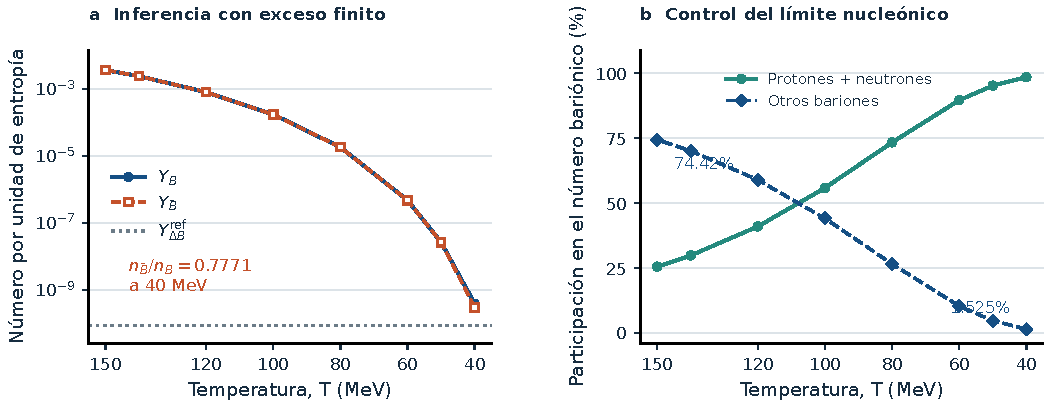
\includegraphics[width=.99\textwidth]{figures/fig05_inverse_es.pdf}
\caption{Resultados propios que responden al objetivo retrospectivo. (a) Rendimientos de bariones y antibariones inferidos con PDG2025 y el exceso publicado como condición de entrada. Las curvas casi coinciden a temperaturas altas; su diferencia aumenta en proporción al total al enfriar. La línea gris es la condición externa conservada. (b) Participación de protones y neutrones, y de los restantes bariones, en el control simétrico. Estas participaciones se calcularon aquí; el contraste con la literatura utiliza la aproximación nucleónica de Satarov et al. (2013). Los puntos son estados de equilibrio a temperaturas elegidas, sin constituir una trayectoria cinética medida.}
\label{fig:inverse}
\end{figure*}

\subsection{Cantidades al variar la temperatura de partida}
La referencia de transición de 156.5 MeV correspondió a $1.8161\times10^{12}$ K. Evaluado con las mismas condiciones inversas, PDG2025 dio aproximadamente $2.6575\times10^{37}$ bariones y la misma densidad redondeada de antibariones por cm$^3$. El exceso fue $4.8753\times10^{29}$ cm$^{-3}$, con $\mu_B/T=9.1749\times10^{-9}$. El total, $5.3150\times10^{37}$ cm$^{-3}$, superó en 54.31\% el resultado a 150 MeV. El rendimiento por entropía aumentó 26.95\%, hasta $9.4772\times10^{-3}$, lo que distinguió el cambio de población del cambio de normalización. La Tabla~\ref{tab:initialT} contiene los puntos de sensibilidad. El resultado a 156.5 MeV es nuestra evaluación HRG en una temperatura de referencia publicada, sin convertirla en una medición del inicio de aniquilación.

\begin{table*}[t]\centering\small
\caption{Sensibilidad propia a la temperatura de partida, con PDG2025 y la misma condición neta. La referencia de transición es $156.5\pm1.5$ MeV (HotQCD, 2019); 150 MeV se conserva como inicio de la malla principal. El intervalo cercano a la transición no representa una incertidumbre completa del HRG ni un inicio de aniquilación medido.}\label{tab:initialT}
\setlength{\tabcolsep}{11pt}\renewcommand{\arraystretch}{1.14}
\begin{tabular}{rrrrr}\toprule
$T$ (MeV) & $n_B$ (${\rm cm^{-3}}$) & $n_{\bar B}$ (${\rm cm^{-3}}$) & $\Delta n_B$ (${\rm cm^{-3}}$) & $Y_\Sigma$ \\ \midrule
150 & $1.722\times10^{37}$ & $1.722\times10^{37}$ & $4.011\times10^{29}$ & 0.007465 \\
155 & $2.410\times10^{37}$ & $2.410\times10^{37}$ & $4.660\times10^{29}$ & 0.008991 \\
156.5 & $2.657\times10^{37}$ & $2.657\times10^{37}$ & $4.875\times10^{29}$ & 0.009477 \\
158 & $2.926\times10^{37}$ & $2.926\times10^{37}$ & $5.100\times10^{29}$ & 0.009976 \\
\bottomrule\end{tabular}\end{table*}


\subsection{Información recuperable de la abundancia actual}
El mapa de la ecuación~\eqref{eq:rank} tuvo rango uno para dos componentes desconocidos y dirección nula $(1,1)$. Los cuatro ejemplos con totales de 0.1, 1, 10 y 100 veces el total inicial conservaron algebraicamente $Y_B-Y_{\bar B}=8.6932\times10^{-11}$, equivalente a la misma entrada $\eta=6.12\times10^{-10}$. Por tanto, el exceso presente por sí solo no identificó una cantidad inicial única de pares. La relación de equilibrio a una temperatura especificada aportó la información adicional empleada en la reconstrucción anterior.

\subsection{Contraste cuantitativo con el límite nucleónico publicado}
La evaluación propia de la ecuación~\eqref{eq:nucleonMB} dio $n_p+n_n=4.4080\times10^{36}$ cm$^{-3}$ a 150 MeV en la aproximación de Maxwell-Boltzmann. La suma de Fermi-Dirac fue $4.4054\times10^{36}$ cm$^{-3}$: la diferencia relativa fue 0.05916\%. Los nucleones aportaron 25.5799\% del total bariónico del HRG simétrico y los restantes bariones, 74.4201\%. A 40 MeV la participación nucleónica alcanzó 98.4745\% (Tabla~\ref{tab:nucleoncontrast}). Estas cifras son resultados de nuestros cálculos sobre la aproximación y el catálogo declarados; no son poblaciones medidas ni cifras tabuladas por los autores comparados.

\begin{table*}[t]\centering\small
\caption{Contraste calculado con el límite nucleónico de Satarov et al. (2013), generalizado a masas distintas de $p$ y $n$. Todas las columnas numéricas son resultados propios a $\mu_B=0$. $\delta_{\rm MB}$ expresa $100(n_N^{\rm MB}/n_N^{\rm FD}-1)$; la participación de otros bariones usa el total HRG con Fermi-Dirac.}\label{tab:nucleoncontrast}
\setlength{\tabcolsep}{8pt}\renewcommand{\arraystretch}{1.14}
\begin{tabular}{rrrrr}\toprule
$T$ (MeV) & $n_N^{\rm MB}$ (${\rm cm^{-3}}$) & $n_B^{\rm HRG}$ (${\rm cm^{-3}}$) & Otros bariones (\%) & $\delta_{\rm MB}$ (\%) \\ \midrule
150 & $4.408\times10^{36}$ & $1.722\times10^{37}$ & 74.4201 & 0.05916 \\
140 & $2.498\times10^{36}$ & $8.354\times10^{36}$ & 70.1063 & 0.03814 \\
120 & $6.261\times10^{35}$ & $1.525\times10^{36}$ & 58.9552 & 0.01268 \\
100 & $9.612\times10^{34}$ & $1.720\times10^{35}$ & 44.1293 & 0.002696 \\
80 & $6.342\times10^{33}$ & $8.643\times10^{33}$ & 26.6153 & $2.623\times10^{-4}$ \\
60 & $7.938\times10^{31}$ & $8.859\times10^{31}$ & 10.3973 & $5.341\times10^{-6}$ \\
50 & $2.591\times10^{30}$ & $2.722\times10^{30}$ & 4.7824 & $2.357\times10^{-7}$ \\
40 & $1.664\times10^{28}$ & $1.690\times10^{28}$ & 1.5255 & $2.176\times10^{-9}$ \\
\bottomrule\end{tabular}\end{table*}


\subsection{Control simétrico del inventario inicial}
Para verificar el efecto de imponer simetría, se repitió el cálculo con $\mu_B=0$. El inventario PDG2025 produjo 443 especies de partícula activas: 146 bariónicas, 146 antibariónicas y 151 mesónicas. Esos recuentos describieron tipos de partícula; las poblaciones se obtuvieron mediante la ecuación~\eqref{eq:number}. A $T_i=150$ MeV, el cálculo propio dio
\begin{align}
n_B^{\rm eq}&=1.7222003\times10^{37}\ {\rm cm^{-3}},\\
n_{\bar B}^{\rm eq}&=1.7222003\times10^{37}\ {\rm cm^{-3}},\\
n_\Sigma^{\rm eq}&=3.4444006\times10^{37}\ {\rm cm^{-3}}.
\label{eq:initialpopulation}
\end{align}
Por cada cm$^3$ físico de plasma a esa temperatura, el número medio reconstruido fue $1.7222\times10^{37}$ bariones y el mismo número de antibariones. La contabilidad simétrica correspondió a $1.7222\times10^{37}$ pares potenciales por cm$^3$. Las densidades mesónica y fotónica fueron, respectivamente, $2.4649\times10^{38}$ y $1.0700\times10^{38}$ cm$^{-3}$.

Entre las especies de partícula nucleónicas, se obtuvieron $n_p=n_{\bar p}=2.2103\times10^{36}$ y $n_n=n_{\bar n}=2.1951\times10^{36}$ cm$^{-3}$. Protones y neutrones sumaron 25.58\% de la densidad de todos los bariones de ese inventario a 150 MeV. Estos valores correspondieron a las poblaciones primarias de equilibrio, antes de propagar desintegraciones de resonancias. La identidad $n_B=n_{\bar B}$ dio exceso neto cero en el control simétrico.

\subsection{Secuencia del control simétrico durante el enfriamiento}
La Tabla~\ref{tab:populations} contiene la reconstrucción en las ocho temperaturas. A 40 MeV se obtuvieron $n_B=n_{\bar B}=1.6896\times10^{28}$ cm$^{-3}$ y $n_\Sigma=3.3791\times10^{28}$ cm$^{-3}$. El rendimiento total disminuyó de $Y_\Sigma^{\rm eq}=7.4653\times10^{-3}$ a $6.8756\times10^{-10}$, una reducción de 7.0357 órdenes de magnitud (Figura~\ref{fig:populations}). El número físico por cm$^3$ y el rendimiento por entropía se conservaron como magnitudes distintas.

\begin{table*}[t]\centering\small
\caption{Densidades numéricas de equilibrio reconstruidas con PDG2025, a potenciales químicos nulos. La densidad de cada lado se muestra en la segunda columna; el total incluye ambos. $Y_\Sigma=n_\Sigma/s_{\rm tot}$ separa la supresión térmica de la dilución. $\mathcal Q=Y_\Sigma/Y_{\Delta B}^{\rm ref}$ usa el exceso cosmológico como entrada externa. Son poblaciones instantáneas calculadas, sin contabilizar reacciones de regeneración o aniquilación.}\label{tab:populations}
\setlength{\tabcolsep}{12pt}\renewcommand{\arraystretch}{1.14}
\begin{tabular}{rrrrr}\toprule
$T$ (MeV) & $n_B=n_{\bar B}$ (${\rm cm^{-3}}$) & $n_\Sigma$ (${\rm cm^{-3}}$) & $Y_\Sigma$ & $\mathcal Q$ \\ \midrule
150 & $1.722\times10^{37}$ & $3.444\times10^{37}$ & 0.007465 & $8.587\times10^{7}$ \\
140 & $8.354\times10^{36}$ & $1.671\times10^{37}$ & 0.004887 & $5.622\times10^{7}$ \\
120 & $1.525\times10^{36}$ & $3.051\times10^{36}$ & 0.001634 & $1.880\times10^{7}$ \\
100 & $1.720\times10^{35}$ & $3.441\times10^{35}$ & $3.506\times10^{-4}$ & $4.033\times10^{6}$ \\
80 & $8.643\times10^{33}$ & $1.729\times10^{34}$ & $3.687\times10^{-5}$ & $4.241\times10^{5}$ \\
60 & $8.859\times10^{31}$ & $1.772\times10^{32}$ & $9.595\times10^{-7}$ & $1.104\times10^{4}$ \\
50 & $2.722\times10^{30}$ & $5.443\times10^{30}$ & $5.331\times10^{-8}$ & 613.2 \\
40 & $1.690\times10^{28}$ & $3.379\times10^{28}$ & $6.876\times10^{-10}$ & 7.909 \\
\bottomrule\end{tabular}\end{table*}

\begin{figure*}[t]
\centering
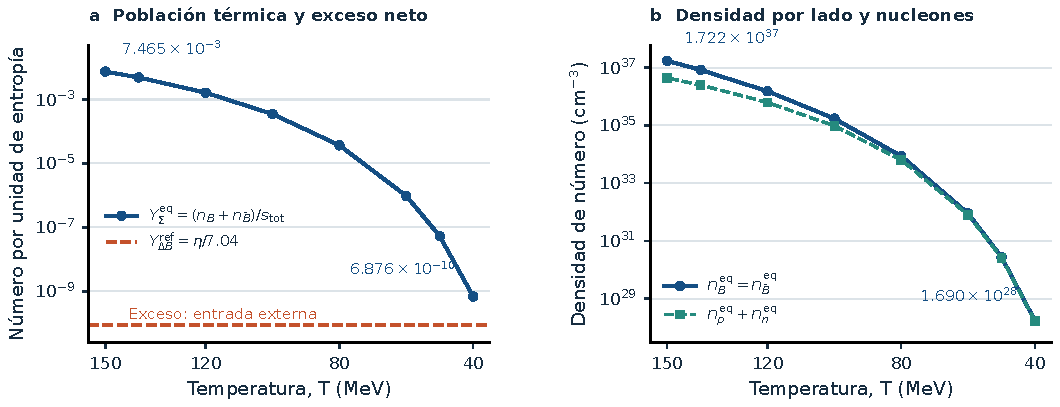
\includegraphics[width=.99\textwidth]{figures/fig04_populations_es.pdf}
\caption{Reconstrucción propia de las poblaciones numéricas con PDG2025. (a) Rendimiento térmico total $Y_\Sigma^{\rm eq}$ y exceso neto de referencia $Y_{\Delta B}^{\rm ref}=8.6932\times10^{-11}$. La línea del exceso utiliza una normalización cosmológica externa; la curva azul se calculó con el inventario HRG. (b) Densidad de cada lado simétrico y contribución de protones y neutrones. En el control simétrico, cada curva de antipartículas coincide con la de sus partículas. Los ejes siguen el enfriamiento y los segmentos guían la lectura. Son poblaciones instantáneas de equilibrio, sin contabilizar eventos acumulados de aniquilación o regeneración.}
\label{fig:populations}
\end{figure*}


\subsection{Contraste a temperatura fija}
Las tres listas ampliadas produjeron fracciones que disminuyeron en toda la malla al bajar la temperatura (Tabla~\ref{tab:comparison}; Figura~\ref{fig:comparison}). Con PDG2025 se obtuvo
\begin{align}
\fB(150\ {\rm MeV})&=0.08454533,\\
\fB(40\ {\rm MeV})&=1.7970078\times10^{-8}.
\end{align}
El primer valor equivale a 8.4545\%, mientras que el segundo equivale a $1.7970\times10^{-6}\%$.

\begin{table*}[t]\centering\footnotesize
\caption{Comparación a temperatura fija de la fracción de entropía barión-antibarión. Las cuatro columnas de $f$ son fracciones adimensionales; las dos últimas se expresan en porcentaje. La referencia reducida fue transcrita del manuscrito previo; las columnas PDG se calcularon en esta auditoría con el mismo plasma ligero. El cociente descriptivo se evaluó antes del redondeo del resultado PDG.}\label{tab:comparison}
\setlength{\tabcolsep}{9pt}\renewcommand{\arraystretch}{1.14}
\begin{tabular}{rrrrrrr}\toprule
$T$ (MeV) & $f_{\mathrm{previo}}$ & $f_{\mathrm{PDG2014}}$ & $f_{\mathrm{PDG2020}}$ & $f_{\mathrm{PDG2025}}$ & $100R$ & $100d$ \\ \midrule
150 & 0.06208 & 0.08351 & 0.08459 & 0.08455 & 73.43 & 26.57 \\
140 & 0.04328 & 0.05633 & 0.05695 & 0.05693 & 76.02 & 23.98 \\
120 & 0.01686 & 0.02018 & 0.02032 & 0.02032 & 82.97 & 17.03 \\
100 & 0.004305 & 0.004734 & 0.00475 & 0.00475 & 90.64 & 9.36 \\
80 & $5.464\times10^{-4}$ & $5.655\times10^{-4}$ & $5.661\times10^{-4}$ & $5.661\times10^{-4}$ & 96.52 & 3.48 \\
60 & $1.782\times10^{-5}$ & $1.795\times10^{-5}$ & $1.795\times10^{-5}$ & $1.795\times10^{-5}$ & 99.26 & 0.74 \\
50 & $1.148\times10^{-6}$ & $1.152\times10^{-6}$ & $1.152\times10^{-6}$ & $1.152\times10^{-6}$ & 99.67 & 0.33 \\
40 & $1.795\times10^{-8}$ & $1.797\times10^{-8}$ & $1.797\times10^{-8}$ & $1.797\times10^{-8}$ & 99.89 & 0.11 \\
\bottomrule\end{tabular}\end{table*}

\begin{figure*}[t]
\centering
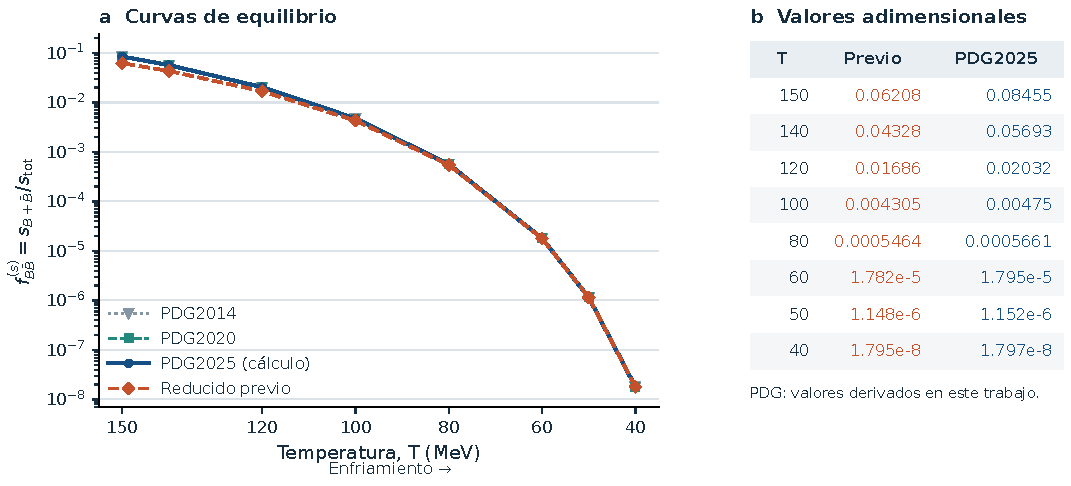
\includegraphics[width=.99\textwidth]{figures/fig01_comparison_es.pdf}
\caption{Fracción de entropía del sector barión-antibarión a potenciales químicos nulos. (a) Comparación semilogarítmica de la referencia reducida y de los tres cálculos independientes con listas de Thermal-FIST basadas en PDG2014, PDG2020 y PDG2025. El eje horizontal sigue el enfriamiento de izquierda a derecha. (b) Valores adimensionales de la referencia y del cálculo PDG2025 en las ocho temperaturas. Todas las curvas PDG son resultados derivados de este cálculo, con anchos de resonancia nulos y el mismo sector ligero en el denominador; no son mediciones externas. Los segmentos unen los puntos calculados y sirven de guía visual.}
\label{fig:comparison}
\end{figure*}

A 150 MeV, la referencia previa de 6.208\% se situó 2.2465 puntos porcentuales por debajo del cálculo PDG2025. El cociente $R$ fue 0.73428 y el déficit relativo, 26.57\%. Al enfriar, $100R$ aumentó hasta 90.64\% a 100 MeV, 99.26\% a 60 MeV y 99.89\% a 40 MeV (Figura~\ref{fig:convergence}). La variación máxima entre las tres listas en la malla se presentó a 150 MeV: 0.10775 puntos porcentuales. Sus porcentajes allí fueron 8.3509, 8.4586 y 8.4545\% para PDG2014, PDG2020 y PDG2025, respectivamente.

\begin{figure*}[t]
\centering
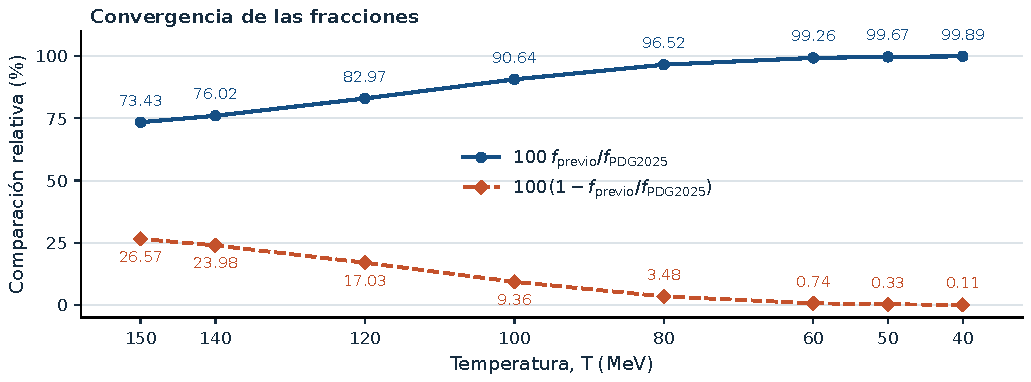
\includegraphics[width=.99\textwidth]{figures/fig02_convergence_es.pdf}
\caption{Contraste relativo entre la referencia reducida previa y el cálculo PDG2025. Los puntos azules muestran $100R=100f_{\rm previo}/f_{25}$; los naranjas, su complemento $100d=100(1-R)$. Las etiquetas contienen los valores porcentuales calculados antes del redondeo de $f_{25}$, usando los cuatro dígitos significativos disponibles para la referencia previa. Estas cantidades miden concordancia numérica entre fracciones de equilibrio; no son probabilidades de validación ni porcentajes de pares aniquilados.}
\label{fig:convergence}
\end{figure*}

\subsection{Forma de las series}
La correlación entre los logaritmos de las ocho fracciones fue $r_{\log}=0.9999233$, con $\mathrm{RMSE}_{\log}=0.0714338$. El cociente entre los extremos fue $2.89143\times10^{-7}$ para la referencia reducida y $2.12550\times10^{-7}$ para PDG2025. Las disminuciones correspondientes fueron de 6.539 y 6.673 órdenes de magnitud. La correlación de rangos de Spearman fue $\rho_S=1$, consistente con el orden monotónico compartido por ambas series. Estas métricas resumieron la forma y el contraste de amplitud de las series en la malla elegida.

\subsection{Densidades y efecto del denominador}
Con PDG2025 a 150 MeV se obtuvieron las siguientes densidades:
\begin{align}
\sB&=2.9972147\times10^{-3}\ {\rm GeV^3},\\
s_{\rm mes}&=1.1626411\times10^{-2}\ {\rm GeV^3},\\
\shad&=1.4623626\times10^{-2}\ {\rm GeV^3},\\
\sL&=2.0827352\times10^{-2}\ {\rm GeV^3},\\
\stot&=3.5450978\times10^{-2}\ {\rm GeV^3}.
\end{align}
La partición de $\stot$ fue 8.4545\% bariones y antibariones, 32.7957\% mesones y 58.7497\% sector ligero. Al utilizar sólo $\shad$ como denominador, la fracción del mismo numerador fue 20.4957\% (Figura~\ref{fig:denominator}).

\begin{figure*}[t]
\centering
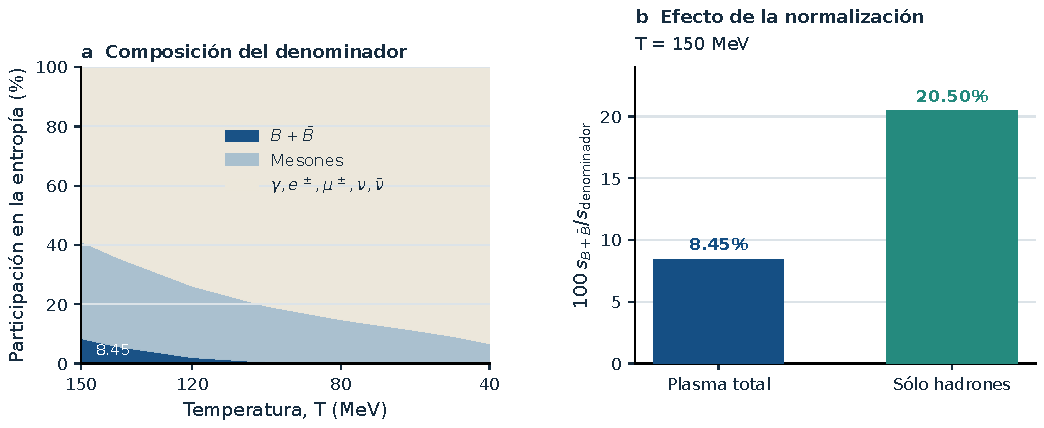
\includegraphics[width=.99\textwidth]{figures/fig03_denominator_es.pdf}
\caption{Efecto de la definición de la entropía total en el cálculo PDG2025. (a) Participación de bariones y antibariones, mesones y sector ligero en $\stot$ a las ocho temperaturas; las áreas entre puntos sólo guían la lectura. (b) El mismo numerador $\sB$ a 150 MeV representa 8.45\% de la entropía del plasma considerado y 20.50\% de la entropía exclusivamente hadrónica. El cambio se debe a la normalización, no a una población bariónica diferente. La figura representa composición instantánea de equilibrio, sin identificar el destino individual de productos de aniquilación.}
\label{fig:denominator}
\end{figure*}

\subsection{Escala del residuo y conexión con H y He}
Al normalizar por el exceso externo $\YB^{\rm ref}=8.6932\times10^{-11}$, se obtuvo $\mathcal Q(150)=8.5875\times10^7$ y $\mathcal Q(40)=7.9092$. Por cada unidad de número bariónico neto de referencia, la población simétrica inicial representó $4.2937\times10^7$ bariones y el mismo número de antibariones. Esta comparación utilizó una normalización comóvil común. A 40 MeV la población total simétrica de equilibrio aún fue 7.91 veces ese exceso; ese extremo de la malla no correspondió a un residuo final calculado.

Con las entradas observacionales y las ecuaciones~\eqref{eq:today} y \eqref{eq:hydrogen} se obtuvieron los valores de la Tabla~\ref{tab:present}. La densidad bariónica media inferida fue $(2.514\pm0.017)\times10^{-7}$ cm$^{-3}$, equivalente a $0.2514\pm0.0017$ unidades bariónicas por m$^3$. Coincidió, al redondeo de entradas, con el valor de referencia $(2.515\pm0.017)\times10^{-7}$ cm$^{-3}$ compilado por \citet{Groom2025}. Ambas conversiones compartieron la normalización del CMB.

\begin{table}[t]
\centering\small
\caption{Conversiones calculadas a partir de las entradas cosmológicas publicadas. Las incertidumbres provienen de propagación de entradas a primer orden, sin incluir errores físicos del HRG. H, He y D indican una composición primordial equivalente a la densidad media actual; no un censo de átomos neutros actuales.}
\label{tab:present}
\setlength{\tabcolsep}{3pt}\renewcommand{\arraystretch}{1.18}
\begin{tabular}{lr}\toprule
Magnitud & Densidad (${\rm cm^{-3}}$)\\\midrule
Fotones CMB & $410.73\pm0.27$\\
Número bariónico neto & $(2.514\pm0.017)\times10^{-7}$\\
Núcleos de H & $(1.898\pm0.015)\times10^{-7}$\\
Núcleos de $^4$He & $(1.540\pm0.021)\times10^{-8}$\\
Núcleos de D & $(4.760\pm0.066)\times10^{-12}$\\
\bottomrule\end{tabular}
\end{table}

La secuencia retrospectiva fue: abundancia presente, condición de conservación del exceso, propiedades del inventario HRG, temperatura elegida y solución de las poblaciones tempranas. Las conversiones H/He/D describieron la referencia cosmológica usada, sin convertirse en predicciones independientes del HRG.

\subsection{Controles numéricos y químicos}
Duplicar el número de términos de la serie no alteró las fracciones al nivel de precisión aritmética registrado. Las integrales independientes cumplieron el criterio de $10^{-8}$ para todas las especies de partícula y temperaturas verificadas. Las densidades de número verificadas mediante integrales independientes difirieron de las sumas en menos de $5\times10^{-16}$ en la precisión registrada. Se exportaron 3544 registros, correspondientes a 443 especies de partícula en ocho temperaturas. La aproximación de electrones sin masa sobreestimó su propia entropía en $1.26\times10^{-6}$ a 150 MeV y $1.77\times10^{-5}$ a 40 MeV, en términos relativos.

La solución inversa cerró la condición neta con error relativo máximo de $2.23\times10^{-15}$ en las tres listas. El cambio al duplicar los términos fue menor que $4.5\times10^{-16}$. Los excesos nucleónicos calculados mediante integrales independientes coincidieron con las sumas dentro de $3.83\times10^{-13}$ en términos relativos. A 40 MeV, incluir el exceso finito aumentó la densidad total de bariones y antibariones en 0.7961\% respecto del control simétrico. Los archivos de validación separaron esta reconstrucción de los controles a potencial nulo.

\section{Discusión}
\subsection{Respuesta al objetivo de reconstrucción}
Los resultados permiten una respuesta condicionada y cuantitativa: las propiedades de las especies de partícula y la abundancia neta observada, junto con una temperatura y un modelo de equilibrio explícitos, permitieron reconstruir por separado bariones y antibariones. La condición inversa incorporó el exceso publicado en el cálculo, en lugar de limitarse a compararlo después con una población simétrica. A 150 MeV se infirieron aproximadamente $1.7222\times10^{37}$ partículas por cm$^3$ de cada lado, con una pequeña diferencia de $4.0110\times10^{29}$ cm$^{-3}$. A 40 MeV, la misma condición neta distinguió $1.9166\times10^{28}$ bariones de $1.4894\times10^{28}$ antibariones por cm$^3$.

La prueba de rango precisó qué información procede del presente. La abundancia neta fija una diferencia; añadir el mismo número de partículas y antipartículas no la modifica. Por ello, las masas y la presencia actual, sin condiciones térmicas adicionales, no determinan cuántos pares existieron. El HRG a temperatura especificada aporta esa relación adicional. La reconstrucción obtenida es una inferencia bajo supuestos comprobables, y no la recuperación única de un registro histórico perdido.

El extremo superior de 150 MeV es el punto inicial elegido para nuestros cálculos dentro del régimen hadrónico considerado. No se identificó una fecha universal en la que comenzara la aniquilación de todas las especies de partícula. Hablar de cantidades \emph{reconstruidas} es preciso; un total de eventos \emph{regenerados} requiere resolver las reacciones inversas en el tiempo.

La amplitud entre las tres listas para la densidad total a 150 MeV fue 1.185\% del valor PDG2025. La sensibilidad a la temperatura de partida fue mayor: cambiar de 150 a 156.5 MeV elevó el total físico reconstruido 54.31\% y su rendimiento 26.95\%. Esto exige declarar la temperatura junto a cada cantidad. La referencia de \citet{Bazavov2019} aporta una escala física para la formación de hadrones; justificar un inicio cinético específico todavía requiere las tasas de reacción y la expansión. Cerca de esa transición, verificar el HRG frente a la ecuación de estado de QCD es necesario para atribuir precisión física al conteo.

\subsection{Qué concuerda con lo publicado}
Nuestro contraste con el límite nucleónico de \citet{Satarov2013} mostró que la aproximación de Maxwell-Boltzmann y la evaluación de Fermi-Dirac difirieron apenas 0.05916\% para protones y neutrones a 150 MeV. La diferencia entre nucleones solos y todo el inventario fue mucho mayor: los otros bariones aportaron 74.42\% del total a esa temperatura, 44.13\% a 100 MeV y 1.525\% a 40 MeV. Estas proporciones calculadas aquí concuerdan con la importancia de las resonancias pesadas a temperaturas altas señalada por esos autores. El contraste identifica qué parte de la diferencia se debe al inventario y qué parte a la aproximación de distribución.

La comparación no reprodujo su evolución cinética ni sus correcciones de interacción. Tampoco ofrece una verificación observacional directa de las densidades tempranas. La literatura aportó una aproximación y un comportamiento de referencia; nuestro código evaluó sus magnitudes bajo los supuestos comunes declarados. A 40 MeV la población total inferida todavía fue 7.97 veces el exceso neto, por lo que el extremo inferior tampoco fue una abundancia residual final.

Las curvas de entropía conservaron la disminución de la referencia reducida y concentraron su mayor discrepancia a 150 MeV. En el límite no relativista, con $x_i=m_i/T\gg1$,
\begin{equation}
\frac{s_i}{T^3}\simeq
\frac{g_i}{(2\pi)^{3/2}}x_i^{3/2}
\left(x_i+\frac{5}{2}\right)e^{-x_i}.
\label{eq:asymptotic}
\end{equation}
Esta supresión explica la pérdida de contribución de las masas altas al enfriar. La referencia reducida carece de inventario completo y código original, por lo que su comparación conserva el alcance de una transcripción. La correlación alta describe la forma común de las series; no establece exactitud física ni valida una hipótesis de origen de la materia.

\subsection{Aporte propio y alcance de la novedad}
El aporte comprobable fue la reconstrucción numérica explícita con inventarios fijados, la conexión inversa con el exceso actual, el conteo separado de partículas y antipartículas, y los controles reproducibles. Las nuevas tablas y proporciones son resultados de nuestros cálculos. Los mecanismos de aniquilación, las distribuciones térmicas y el uso de HRG ya están establecidos en la literatura \citep{Vovchenko2019,Satarov2013}. El límite de información de una diferencia neta es una propiedad matemática del problema.

No se demostró aquí un mecanismo físico nuevo, una nueva especie de partícula ni una predicción independiente de la asimetría o del hidrógeno actual. La comparación realizada permite evaluar concordancias y diferencias cuantitativas, pero no basta para establecer prioridad o novedad frente a toda la literatura. Esa afirmación requeriría una revisión específica de trabajos previos y un resultado que pudiera distinguirse de sus predicciones bajo condiciones equivalentes.

\subsection{Secuencia hasta las abundancias actuales}
La Tabla~\ref{tab:external} declara el papel de cada referencia. La revisión de BBN de 2025 incorporó mediciones de deuterio, incluida la de \citet{Cooke2018}, y recomendó el promedio usado en nuestra conversión. Primero, $\eta$ fijó el rendimiento neto; segundo, el HRG y la temperatura permitieron reconstruir las poblaciones tempranas; tercero, $\eta$ y la temperatura del CMB dieron la densidad bariónica media actual; finalmente, $Y_p$ y D/H permitieron expresar una composición primordial equivalente de H, He y D.

La densidad equivalente de H, $(1.898\pm0.015)\times10^{-7}$ cm$^{-3}$, depende de esas entradas adicionales. Su cálculo no constituye una predicción nuclear independiente del HRG. La coincidencia de la densidad bariónica con la tabla publicada comprueba la conversión con una entrada CMB compartida. Las abundancias nucleares requieren evolución hasta BBN y una red de reacciones \citep{Fields2025}; el censo de hidrógeno neutro actual requiere además procesamiento estelar e ionización.

\begin{table*}[t]
\centering\small
\caption{Referencias publicadas y papel en la reconstrucción. Las incertidumbres corresponden a las fuentes, con redondeo declarado para $T_{\gamma0}$; los límites FIRAS son a 95\% de confianza. Se distingue una entrada del cálculo de un canal de comparación que no se ajustó en este trabajo.}
\label{tab:external}
\setlength{\tabcolsep}{5pt}\renewcommand{\arraystretch}{1.15}
\begin{tabular}{>{\raggedright\arraybackslash}p{.18\textwidth}>{\raggedright\arraybackslash}p{.23\textwidth}>{\raggedright\arraybackslash}p{.22\textwidth}>{\raggedright\arraybackslash}p{.26\textwidth}}\toprule
Observable & Valor publicado & Fuente & Papel en la reconstrucción\\\midrule
$\eta_{10}$ del CMB & $6.12\pm0.04$ & \citet{Fields2025} & Condición neta de la inferencia inversa.\\
Temperatura CMB actual & $2.7255\pm0.0006$ K & \citet{Fixsen2009}, redondeado & Densidad fotónica y normalización actual.\\
Fracción bariónica en $^4$He & $Y_p=0.245\pm0.003$ & \citet{Fields2025} & Conversión aproximada a H y He.\\
Deuterio primordial & $(2.508\pm0.029)\times10^{-5}$ & \citet{Fields2025} & Conversión aproximada a D.\\
Densidad bariónica actual & $(2.515\pm0.017)\times10^{-7}$ cm$^{-3}$ & \citet{Groom2025} & Comprobación de conversión; entrada CMB compartida.\\
Densidad $\Omega_bh^2$ & $0.02237\pm0.00015$ & \citet{Planck2020} & Referencia externa; no se ajustó un modelo cosmológico.\\
Distorsiones espectrales & $|y|<1.5\times10^{-5}$\newline $|\mu|<9\times10^{-5}$ & \citet{Fixsen1996} & Restricción relevante para una futura inyección energética tardía.\\
\bottomrule\end{tabular}
\end{table*}

El factor 7.04 usa la aproximación estándar de entropía por fotón después de la aniquilación $e^+e^-$. Los cálculos precisos de desacoplamiento de neutrinos incluyen correcciones \citep{Froustey2020}; el factor no se trató como un parámetro medido con incertidumbre en este trabajo.

\subsection{Poblaciones de equilibrio e historial de aniquilación}
En una expansión adiabática, $S_{\rm com}=\stot a^3$ se conserva aproximadamente. Un esquema de evolución con aniquilación y producción inversa es \citep{Satarov2013}
\begin{align}
\dot n_B+3Hn_B&=-\mathcal C,\\
\dot n_{\bar B}+3Hn_{\bar B}&=-\mathcal C,\\
\mathcal C&=\langle\sigma v\rangle
\bigl(n_Bn_{\bar B}-n_B^{\rm eq}n_{\bar B}^{\rm eq}\bigr).
\end{align}
Al restar las ecuaciones se obtiene $\dot{\Delta n}_B+3H\Delta n_B=0$. Esto justifica usar el exceso conservado como vínculo retrospectivo bajo los supuestos adoptados. Obtener eventos acumulados exige integrar por separado producción y pérdida sobre tiempo y volumen. Una sucesión de estados de equilibrio no proporciona esos totales.

\subsection{Limitaciones de la reconstrucción}
Se usaron masas nominales, anchos nulos, un gas ideal y una temperatura común, sin ajustes a datos de red ni incertidumbres de masas, espín e interacciones. La condición neta no resolvió la neutralidad de carga y extrañeza simultáneamente. Los controles verificaron precisión numérica, no la exactitud física de esos supuestos. La cercanía de 150 MeV a la transición exige comprobar las correcciones del modelo antes de asignar errores físicos \citep{Bazavov2012}.

Las incertidumbres cosmológicas sólo se propagaron a las conversiones actuales; las poblaciones inversas usaron entradas centrales. La amplitud entre catálogos es sensibilidad a inventarios correlacionados. El estudio no identificó el inicio cinético, no integró tasas de reacción ni generó la asimetría primordial \citep{Sakharov1967}. Dentro de ese alcance, establece cantidades tempranas condicionadas y una forma explícita de contrastarlas con el conocimiento disponible.

\section{Conclusiones}
El objetivo retrospectivo se respondió bajo condiciones declaradas: las masas de reposo y demás propiedades del inventario HRG, combinadas con el exceso bariónico observado y una temperatura elegida, permitieron reconstruir poblaciones separadas de bariones y antibariones. A 150 MeV se infirieron aproximadamente $1.7222\times10^{37}$ cm$^{-3}$ de cada lado, con exceso de $4.0110\times10^{29}$ cm$^{-3}$. A 40 MeV se distinguieron $1.9166\times10^{28}$ bariones y $1.4894\times10^{28}$ antibariones por cm$^3$. El rendimiento total bajó 7.0323 órdenes de magnitud.

La abundancia actual sola no recuperó una población inicial única: el mapa del exceso tuvo rango uno y conservó cualquier adición igual de partículas y antipartículas. La condición de equilibrio a temperatura fijada fue información adicional necesaria. El contraste con el límite nucleónico publicado cuantificó una participación de otros bariones de 74.42\% a 150 MeV y 1.525\% a 40 MeV, coherente con su supresión térmica.

La referencia publicada $T_c=156.5\pm1.5$ MeV fundamentó una comprobación de la temperatura de partida. A su valor central, el mismo HRG dio $2.6575\times10^{37}$ cm$^{-3}$ por lado al redondeo mostrado, con un total 54.31\% mayor que a 150 MeV. Esta sensibilidad cuantifica la importancia del punto inicial, sin identificarlo con un inicio de aniquilación medido.

Los resultados son una reconstrucción reproducible condicionada, sin demostrar un descubrimiento físico nuevo o un historial único de aniquilación. Las densidades actuales de referencia, $n_{b0}=(2.514\pm0.017)\times10^{-7}$ cm$^{-3}$ y el equivalente primordial de H de $(1.898\pm0.015)\times10^{-7}$ cm$^{-3}$, proceden de conversiones de entradas observacionales. Determinar eventos acumulados, inicio cinético y abundancias nucleares finales requiere tasas de reacción y evolución cosmológica.

\section*{Disponibilidad de datos y código}
El suplemento incluye catálogos fijados y SHA-256; densidades numéricas y de entropía; 3544 registros por especie de partícula y temperatura para el control PDG2025; 24 estados de inferencia inversa y 12 evaluaciones de temperatura inicial; el contraste nucleónico; la prueba de rango; las conversiones cosmológicas; controles numéricos; cinco figuras por idioma y fuentes del manuscrito. Los cálculos se ejecutaron con la implementación Python independiente incluida, utilizando los datos de Thermal-FIST y conservando su licencia original.

\section*{Asistencia en la preparación}
Se utilizó asistencia de inteligencia artificial para organizar la redacción y preparar código, figuras y maquetación. Las sumas, integrales y soluciones inversas descritas se ejecutaron y sus resultados se conservaron. La evaluación científica y la decisión de publicación corresponden al autor.



\onecolumn
\begin{multicols}{2}
\begin{thebibliography}{99}\small
\setlength{\itemsep}{2pt}
\bibitem[Bazavov et al.(2012)]{Bazavov2012}
Bazavov, A., Bhattacharya, T., DeTar, C. E., Ding, H.-T., Gottlieb, S., Gupta, R., Hegde, P., Heller, U. M., Karsch, F., Laermann, E., Levkova, L., Mukherjee, S., Petreczky, P., Schmidt, C., Soltz, R. A., Soeldner, W., Sugar, R., \& Vranas, P. M. (2012).
Fluctuations and correlations of net baryon number, electric charge, and strangeness: A comparison of lattice QCD results with the hadron resonance gas model.
\emph{Physical Review D, 86}, 034509. \doi{10.1103/PhysRevD.86.034509}.

\bibitem[Bazavov et al.(2019)]{Bazavov2019}
Bazavov, A., Ding, H.-T., Hegde, P., Kaczmarek, O., Karsch, F., Karthik, N., Laermann, E., Lahiri, A., Larsen, R., Li, S.-T., Mukherjee, S., Ohno, H., Petreczky, P., Sandmeyer, H., Schmidt, C., Sharma, S., \& Steinbrecher, P. (HotQCD Collaboration). (2019).
Chiral crossover in QCD at zero and non-zero chemical potentials.
\emph{Physics Letters B, 795}, 15--21. \doi{10.1016/j.physletb.2019.05.013}.

\bibitem[Cooke et al.(2018)]{Cooke2018}
Cooke, R. J., Pettini, M., \& Steidel, C. C. (2018).
One percent determination of the primordial deuterium abundance.
\emph{The Astrophysical Journal, 855}(2), 102.
\doi{10.3847/1538-4357/aaab53}.

\bibitem[Fields et al.(2025)]{Fields2025}
Fields, B. D., Molaro, P., \& Sarkar, S. (2025).
Big Bang nucleosynthesis. In \emph{Review of Particle Physics: 2025 update}.
\href{https://pdg.lbl.gov/2025/reviews/rpp2025-rev-bbang-nucleosynthesis.pdf}{PDG review}.

\bibitem[Fixsen(2009)]{Fixsen2009}
Fixsen, D. J. (2009).
The temperature of the cosmic microwave background.
\emph{The Astrophysical Journal, 707}(2), 916--920.
\doi{10.1088/0004-637X/707/2/916}.

\bibitem[Fixsen et al.(1996)]{Fixsen1996}
Fixsen, D. J., Cheng, E. S., Gales, J. M., Mather, J. C., Shafer, R. A., \& Wright, E. L. (1996).
The cosmic microwave background spectrum from the full COBE/FIRAS data set.
\emph{The Astrophysical Journal, 473}, 576--587.
\doi{10.1086/178173}.

\bibitem[Froustey et al.(2020)]{Froustey2020}
Froustey, J., Pitrou, C., \& Volpe, M. C. (2020).
Neutrino decoupling including flavour oscillations and primordial nucleosynthesis.
\emph{Journal of Cosmology and Astroparticle Physics, 2020}(12), 015.
\doi{10.1088/1475-7516/2020/12/015}.

\bibitem[García(2026)]{Garcia2026}
García, A. G. (2026).
\emph{From matter-antimatter annihilation to the baryonic relic: Entropy transfer across the hadronic epoch}
[Unpublished working manuscript, v0.9]. Independent Researcher, Mexico.

\bibitem[Groom and Scott(2025)]{Groom2025}
Groom, D. E., \& Scott, D. (2025).
Astrophysical constants and parameters. In \emph{Review of Particle Physics: 2025 update}, Table 2.1.
\href{https://pdg.lbl.gov/2025/reviews/rpp2025-rev-astrophysical-constants.pdf}{PDG constants table}.

\bibitem[Particle Data Group(2025)]{PDG2025}
Particle Data Group. (2025).
Muon properties. In \emph{Review of Particle Physics: 2025 update}.
\href{https://pdg.lbl.gov/2025/listings/rpp2025-list-muon.pdf}{PDG muon listing}.

\bibitem[Planck Collaboration(2020)]{Planck2020}
Planck Collaboration. (2020).
Planck 2018 results. VI. Cosmological parameters.
\emph{Astronomy \& Astrophysics, 641}, A6.
\doi{10.1051/0004-6361/201833910}.

\bibitem[Robinson and Zyla(2025)]{Robinson2025}
Robinson, D., \& Zyla, P. A. (2025).
Physical constants. In \emph{Review of Particle Physics: 2025 update}, Table 1.1.
\href{https://pdg.lbl.gov/2025/reviews/rpp2025-rev-phys-constants.pdf}{PDG physical constants}.

\bibitem[Sakharov(1967)]{Sakharov1967}
Sakharov, A. D. (1967).
Violation of CP invariance, C asymmetry, and baryon asymmetry of the universe.
\emph{JETP Letters, 5}, 24--27.

\bibitem[Satarov et al.(2013)]{Satarov2013}
Satarov, L. M., Mishustin, I. N., \& Greiner, W. (2013).
Evolution of antibaryon abundances in the early Universe and in heavy-ion collisions.
\emph{Physical Review C, 88}, 024908.
\doi{10.1103/PhysRevC.88.024908}.

\bibitem[Vovchenko and Stoecker(2019)]{Vovchenko2019}
Vovchenko, V., \& Stoecker, H. (2019).
Thermal-FIST: A package for heavy-ion collisions and hadronic equation of state.
\emph{Computer Physics Communications, 244}, 295--310.
\doi{10.1016/j.cpc.2019.06.024}.

\bibitem[Vovchenko and Stoecker(2026)]{TFLists2026}
Vovchenko, V., \& Stoecker, H. (2026).
\emph{Thermal-FIST: PDG2014, PDG2020, and PDG2025 light-and-strange particle lists}
[Data files, repository snapshot \texttt{4086191e9522}].
\href{https://github.com/vlvovch/Thermal-FIST/tree/4086191e952285cd572ba2bbbefb2fdc55401c9b/input/list}{GitHub repository snapshot}.

\end{thebibliography}


\end{multicols}
\end{document}

